\chapter{Розробка макету для тестування датчиків}
\thispagestyle{headings}

\section{Підключення датчиків у Proteus}

\textbf{NTC}\bigskip

Схему макету будемо збирати у Proteus, він дозволяє повноцінно симулювати прості схеми, великим мінусом є той факт, що схема у Proteus працює без похибок та завад, при збірці схеми на макетній платі результати з датчиків будуть дещо відрізнятися.

Arduino не може виміряти опір резистора, тому потрібно зібрати класичну схему з відомим резистором, так невідомим (наш NTC термістор). Опір відомого повинен буде якнайближче до опору невідомого, у нашому випадку NTC термістор має опір 10 кОм, що відповідає 25$^\circ$C. У якості живлення будемо використовувати 3.3 В, адже воно має менше шумів, на реальному макеті також будемо використовувати його як референсне (AREF).

На рис.~\ref{fig:ntc_proteus} можна побачити схему підключення термістора, опір відомого резистора був виміряний на реальній схемі мультиметром, щоб досягти більш точних результатів. Під'єднаємо термістор на A0 пін.

\begin{figure}[ht]
    \centering
    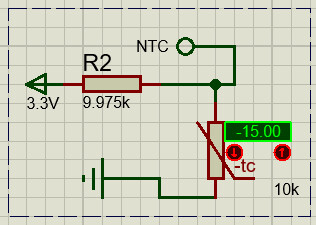
\includegraphics{ntc_proteus.jpg}
    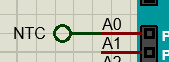
\includegraphics{ntc_proteus2.jpg}
    \caption{Підключення NTC термістора}
    \label{fig:ntc_proteus}
\end{figure}

Щодо роботи з NTC термістором був написаний окремий клас (ліст.~\ref{lst:ntc}) який є спадком базового класу Sensor (ліст.~\ref{lst:sensor_base}), який зчитує напругу та знаючи опір відомого резистора, підраховує опір термістора. Далі за формулою \ref{eq:ntc_beta} отримаємо температуру у градусах Цельсія.\\

\textbf{Термопара К-типу}\bigskip

Як було сказано раніше, термопара дещо відрізняється від підключення інших датчиків, а саме вона є пасивним датчиком та генерує дуже малу напругу при зміні температури (~ 41 мкВ/$^\circ$C), тому потрібно підсилити сигнал за допомогою неінвертуючого операційного підсилювача.

За допомогою потенціометра було підібрано резистор для на зворотного зв'язку (чим менше опір -- тим більше коефіцієнт підсилення). Для підсилення сигналу було обрано подвійний операційний підсилювач LM358N.

\begin{figure}[ht]
    \centering
    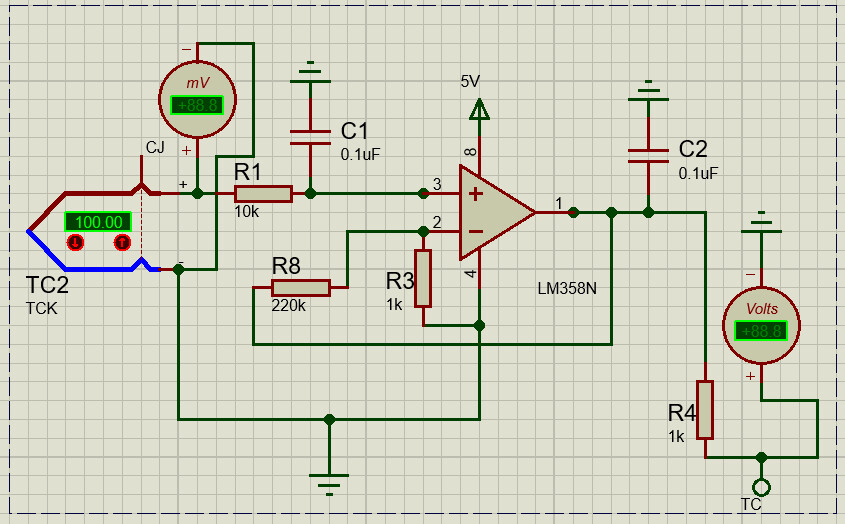
\includegraphics[width=0.8\linewidth]{thermocouple_proteus.jpg}
    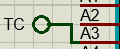
\includegraphics{thermocouple_proteus2.jpg}
    \caption{Підключення термопари К-типу}
    \label{fig:thermocouple_proteus}
\end{figure}

Взагалі це не найкращий вибір мікросхеми для підсилення напруги термопари, адже шумить та сильніше підсилює сигналу відносно до коефіцієнта підсилення. Наприклад можна було встановити спеціалізовану мікросхему AD8495 для термопар К-типу, яка не тільки підсилює сигнал, а ще й виконує компенсацію холодного сплаву за допомогою вбудованого датчика температури. Іншим вибором може бути готова мікросхема від Adafruit -- MAX31865, з якої можна зчитувати конвертовану температуру за допомогою інтерфейсу SPI.

Як було зазначено у формулі \ref{eq:thermocouple}. для того, щоб визначити температуру потрібно знати коефіцієнт підсилювання -- $G = 1+\frac{R_f}{R_{in}} = 1+\frac{220000}{1000} = 221$, але перевіривши експериментальним шляхом було визначено, що це значення не відповідає реальному. Складемо рівняння з невідомим коефіцієнтом підсилення, інші дані відомі після вимірювання. Підставимо ці значення, та знайдемо коефіцієнт підсилення (\ref{eq:tc_gain}). Як можна побачити коефіцієнт значно відрізняється, що могло значно погіршити результати вимірювань. Окрім цього, як було визначено пізніше, операційний підсилювач, також шумить, тобто коли на термопарі мультиметр показує 0 мкВ, на виході підсилювача -- ~5 мВ. АЦП входи Arduino також шумлять, додаючи ~20 мВ. Отже, значення можна скоригувати програмно, віднявши максимум 0.03 В.

\begin{equation}
    \begin{aligned}
        \frac{V}{Ga} + T_{ref} &= T \\
        \frac{0.452}{G\cdot0.000041} + 22.8 &= 57 \\
        G~&\approx~322.35
    \end{aligned}
    \label{eq:tc_gain}
\end{equation}

Табличне значення коефіцієнта Зеєбека -- для термопари К-типу ~41 мкВ/$^\circ$C, температура холодного сплаву -- будемо вимірювати за допомогою NTC термістора та сигнал на виході підсилювача.

Для роботи з термопарою було написано відповідний клас (ліст.~\ref{lst:tc_sensor}), що є нащадком класу Sensor (див. ліст.~\ref{lst:sensor_base}).\\ 

\textbf{DS18B20}\bigskip

На відміну від аналогових датчиків, при підключенні цифрових на повинно виникати складнощів. Вихід даних зазвичай підтягують на живлення використовуючи резистор на ~5 кОм, на це особливо потрібно звертати увагу, коли датчик знаходиться за кілька метрів від мікроконтролера.

На рис.~\ref{fig:ds18b20_proteus} можна побачити підключення цього датчику. Датчик працює по протоколу 1-Wire, для економа часу було використану бібліотеку microDS18B20 для зчитування температури з датчика. Додатковий клас для роботи з цим датчиком та конфігурація у ліст.~\ref{lst:ds18_sensor}.

\begin{figure}[H]
    \centering
    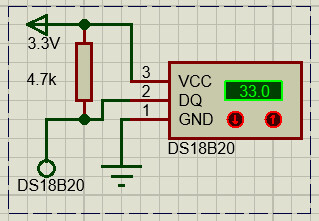
\includegraphics{ds18b20_proteus.jpg}
    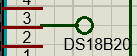
\includegraphics{ds18b20_proteus2.jpg}
    \caption{Підключення датчику DS18B20}
    \label{fig:ds18b20_proteus}
\end{figure}

\textbf{DHT11 та DHT22}\bigskip

Ці датчики також були підключені до живлення 3.3 В, а опір резистора для підтягування був обраний згідно зі специфікацією. На рис.~\ref{fig:dht_proteus} можна побачити підключення цього датчику. Для роботи з датчиками була використана бібліотека ``DHT sensor library'' від Adafruit. Робота з ним також була винесена в окремий клас (ліст.~\ref{lst:dht_sensor}).

\begin{figure}[ht]
    \centering
    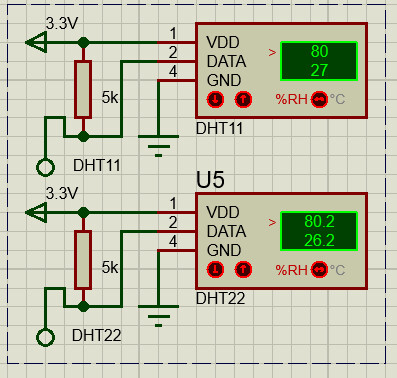
\includegraphics{dht_proteus.jpg}
    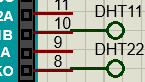
\includegraphics{dht_proteus2.jpg}
    \caption{Підключення датчику DHT11/DHT22}
    \label{fig:dht_proteus}
\end{figure}
\clearpage
\textbf{HTU21D}\bigskip

У моделі Proteus до датчика не можна під'єднати зовнішнє живлення, на макетній платі також будемо використовувати живлення 3.3 В. Цей датчик використовує комунікацію за допомогою I2C шини, беручи до уваги те, що у кожного датчика свій унікальний номер, на цю шину у теорії можна підключити безліч таких датчиків, і окрім цього LCD дисплей, який теж під'єднаємо через I2C шину. На рис.~\ref{fig:htu21_proteus} можна побачити цей датчик з винесеними пінами. Для роботи з датчиком була використана бібліотека HTU2xD\_SHT2x\_Si70xx. Клас для роботи з цим датчиком -- ліст.~\ref{lst:htu21_sensor}.

\begin{figure}[ht]
    \centering
    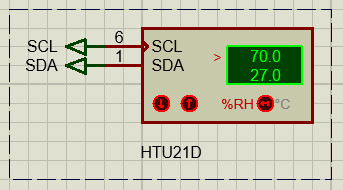
\includegraphics[scale=0.65]{htu21_proteus.jpg}
    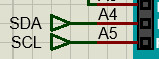
\includegraphics[scale=0.65]{htu21_proteus2.jpg}
    \caption{Підключення датчику HTU21D}
    \label{fig:htu21_proteus}
\end{figure}

\section{Перевірка роботи моделі у Proteus та на макетній платі}

Зібравши усе до купи та під'єднавши LCD дисплей через I2C модуль була написана програмна частина (ліст.~\ref{lst:program}). Очевидно, що інформація відразу з усіх датчиків не поміститься на екран, тому будемо використовувати кнопку для переходу до наступного датчика, яку під'єднаємо за допомогою внутрішньої підтяжки Arduino -- INPUT\_PULLUP.

На рис.~\ref{fig:scheme_test} можна побачити перевірку роботи схеми та програми. Перемикання між екранами здійснюється за допомогою кнопки: один натиск -- наступний датчик, два -- попередній. Робота з кнопкою винесена в окремий клас Button (ліст.~\ref{lst:button}). Використовується Timer (ліст.~\ref{lst:timer}) для запобігання блокування головного циклу програми.

Перевірку зчитування інформації з інших датчиків можна побачити на рис.~\ref{fig:tc_test} -- \ref{fig:dht11_test}.

\begin{figure}[ht]
    \centering
    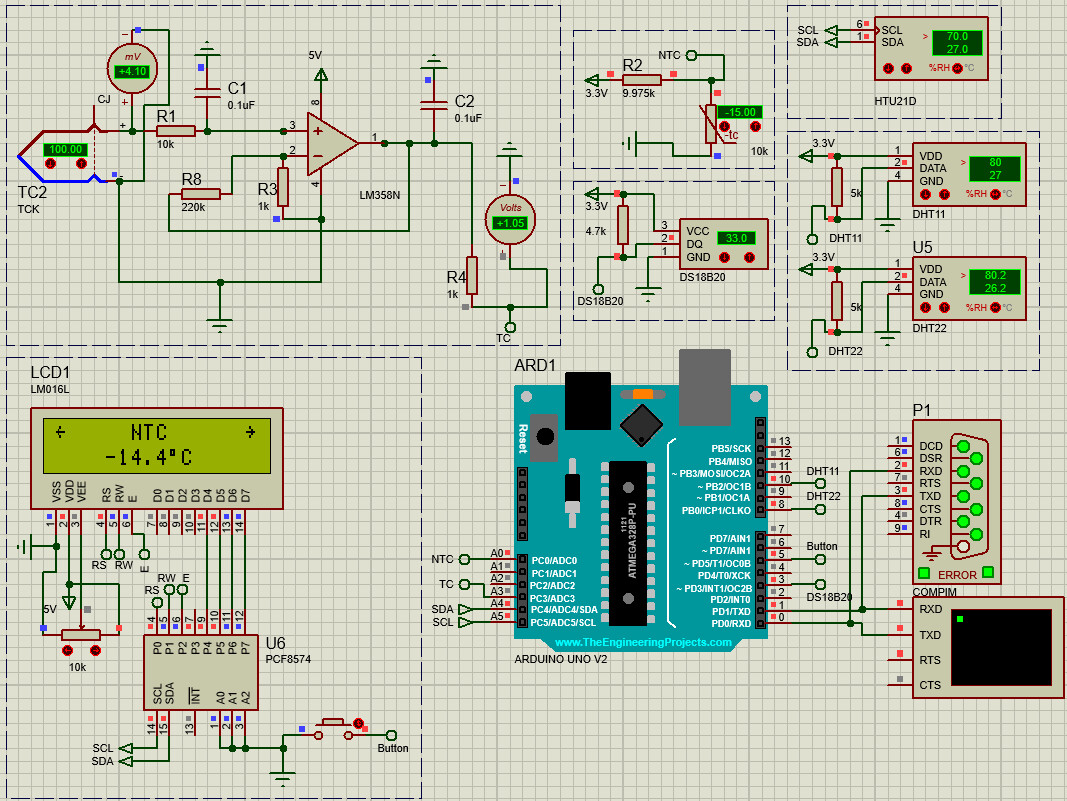
\includegraphics[width=\linewidth]{scheme_test.jpg}
    \caption{}
    \label{fig:scheme_test}
\end{figure}

На макетній платі також була зібрана демонстраційна схема (рис.~\ref{fig:scheme_real}).

\begin{figure}[!hb]
    \centering
    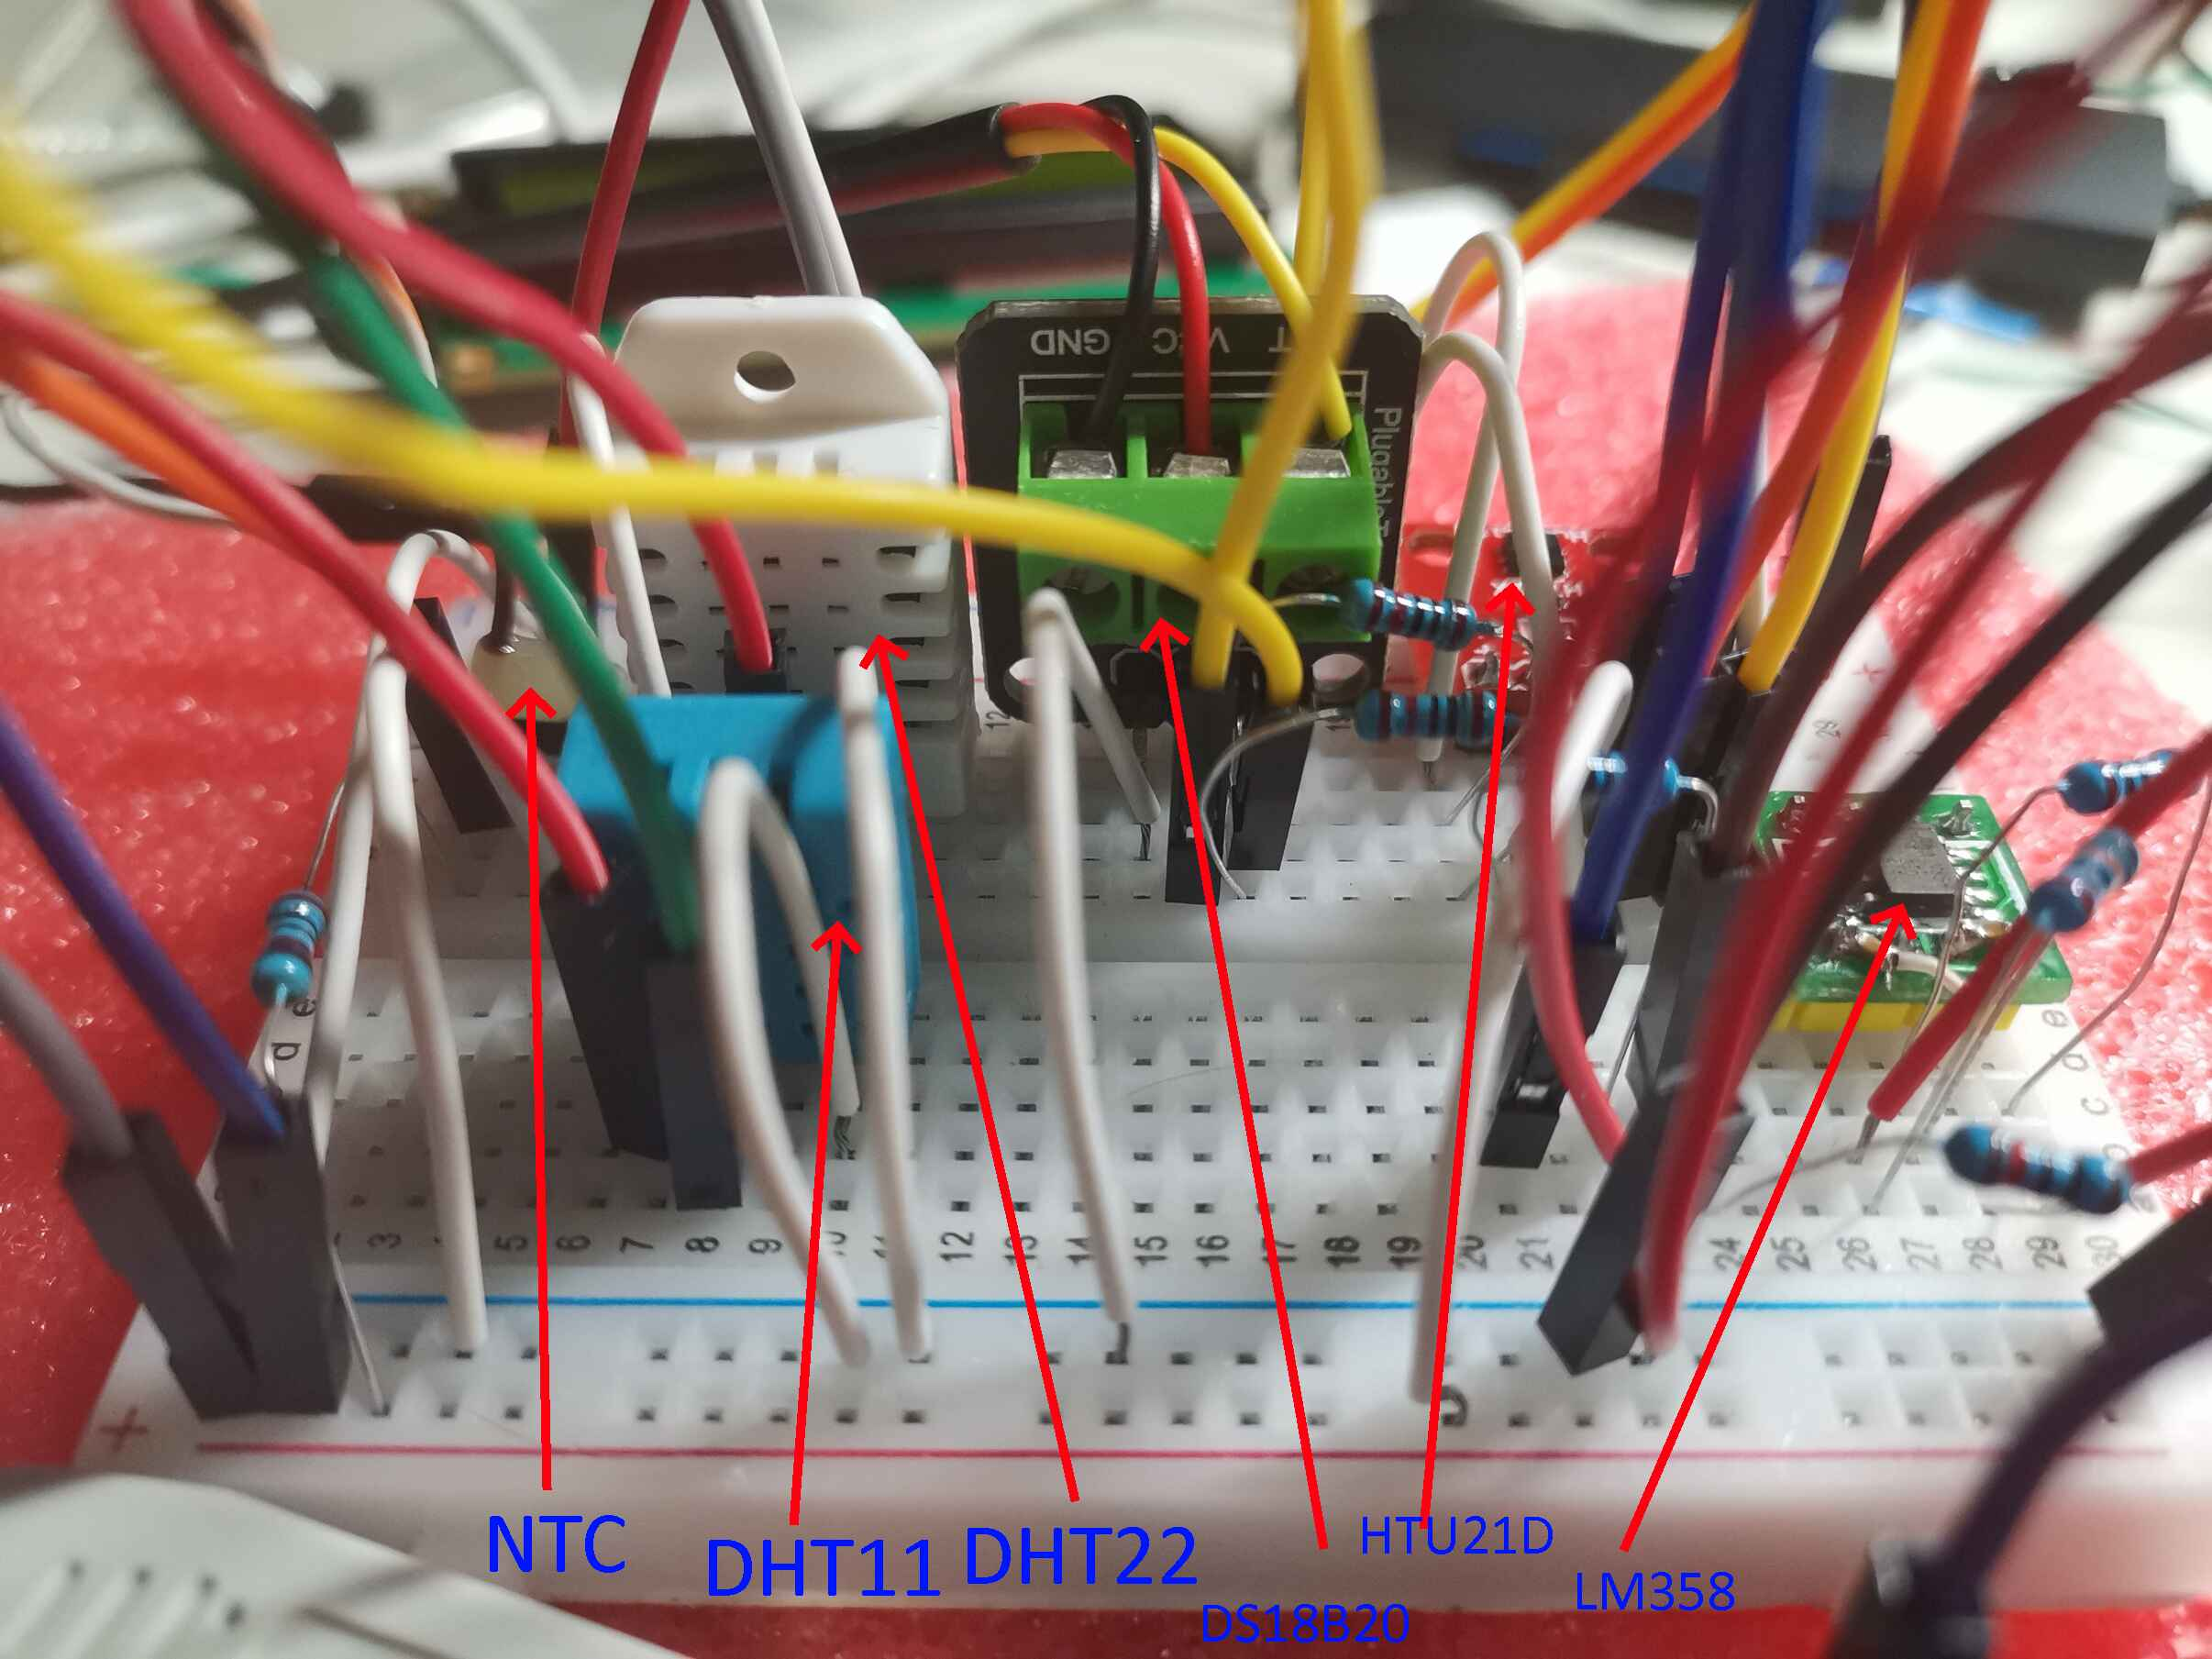
\includegraphics[width=0.75\linewidth]{scheme_real.jpg}
    \caption{Датчики на макетній платі}
    \label{fig:scheme_real}
\end{figure}

Перевірку роботи схеми можна побачити на рис.~\ref{fig:tc_test2} -- \ref{fig:ds18_test2}.\\

\section{Тестування датчиків}

Для перевірки роботи датчиків було побудовано декілька графіків. Як можна побачити на рис.~\ref{fig:plot_normal}, усі датчики видають різні значення при кімнатній температурі, підвищуючи чи знижуючи температуру, але це зовсім не означає, що тільки єдиний датчик, наприклад HTU21D показує правильну температуру. По-перше, сама температура може відрізнятися навіть на відстані декількох сантиметрів, по-друге, в кожного з датчиків у специфікації заявлена можлива похибка.

\begin{figure}[ht]
    \centering
    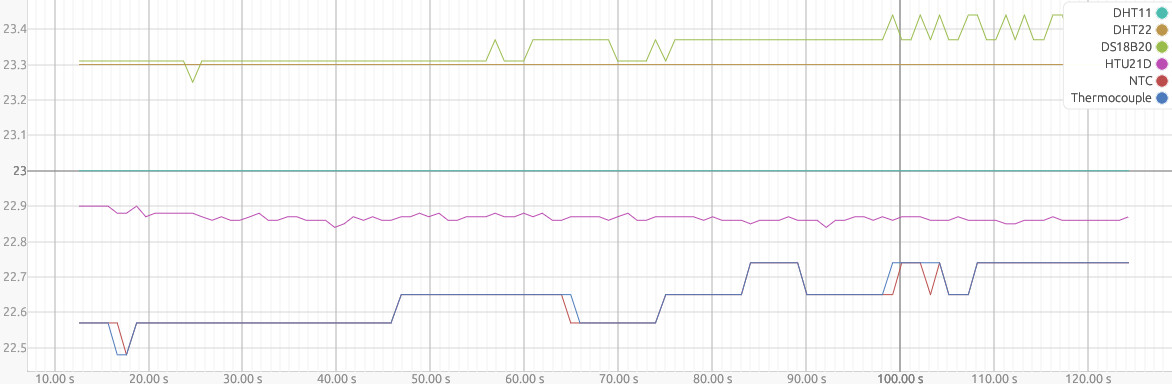
\includegraphics[width=\linewidth]{plot_normal.jpg}
    \caption{Показання датчиків при кімнатній температурі}
    \label{fig:plot_normal}
\end{figure}

У наступному експерименті на відстані ~10 см макетна плата (усі датчики були якнайближче встановлені один до одного) була обдута феном. Як можна побачити на рис.~\ref{fig:plot_hot} цифрові датчики відреагували найповільніше, а у датчиках DHT11/DHT22 спочатку нагрівся корпус, який поступово передав температуру сенсору. DS18B20 показав дещо кращий результат, адже його корпус -- сталь, яка має вищу теплопровідність. HTU21D1 показав кращий результат при спаді температури. Лідером по часу реакції стала термопара, адже її точка з'єднання гарячого та холодного сплаву менша, навіть, за термістор і також зроблена з металу.

\begin{figure}[H]
    \centering
    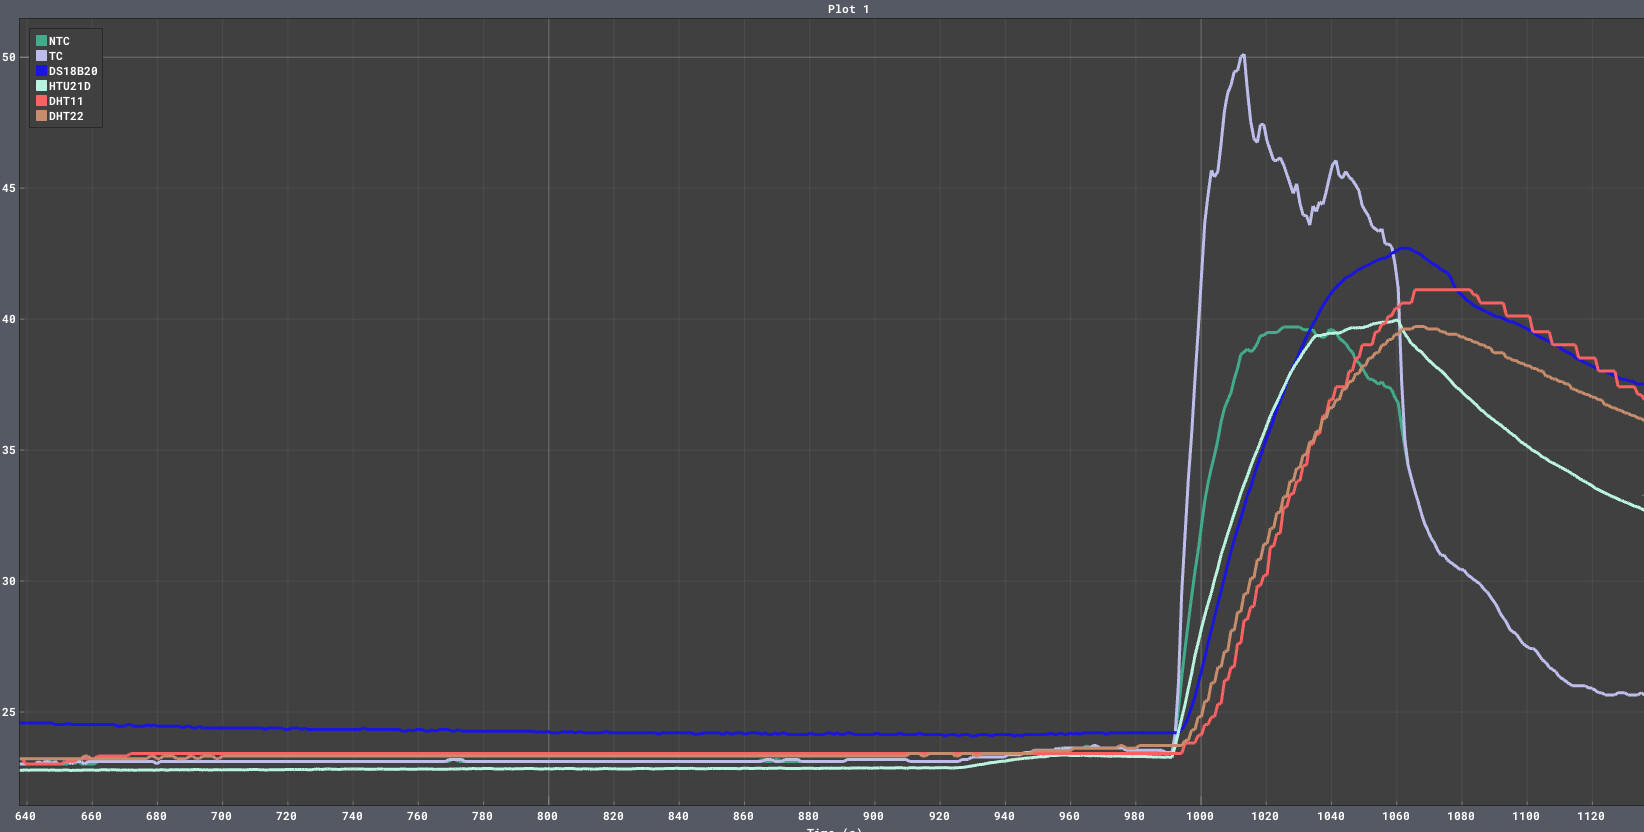
\includegraphics[width=\linewidth]{plot_hot.jpg}
    \caption{Показання датчиків при обдуванні феном}
    \label{fig:plot_hot}
\end{figure}

У теоретичній частині було заявлено, що термопара здатна вимірювати високі температури, перевіримо це за допомогою фену для пайки. Налаштуємо на ньому температуру 350$^\circ$C (рис.~\ref{fig:station}), хоча й і є великі сумніви щодо вбудованого у паяльну станцію датчику. Окрім цього, гаряче повітря буде не рівномірним, тому буде складно досягти саме 350$^\circ$C на термопарі. На термопарі під час нагріву вдалося отримати температуру 348$^\circ$C (рис.~\ref{fig:tc_test3}). На рис.~\ref{fig:plot_station} можна побачити графік нагрітої термопари.

\begin{figure}[ht]
    \centering
    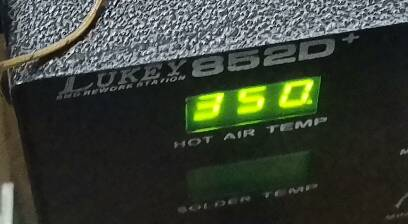
\includegraphics[scale=0.6]{station.jpg}
    \caption{Температура на паяльній станції}
    \label{fig:station}
\end{figure}

\begin{figure}[ht]
    \centering
    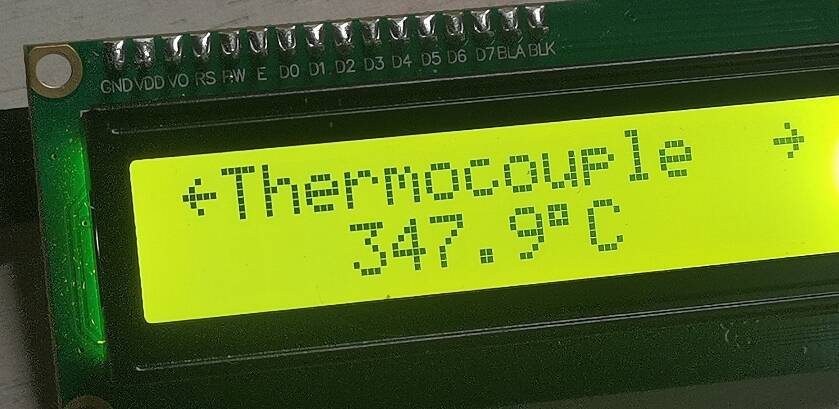
\includegraphics[width=0.4\linewidth]{tc_test3.jpg}
    \caption{Температура на термопарі}
    \label{fig:tc_test3}
    \vspace*{-3em}
\end{figure}

\begin{figure}[ht]
    \centering
    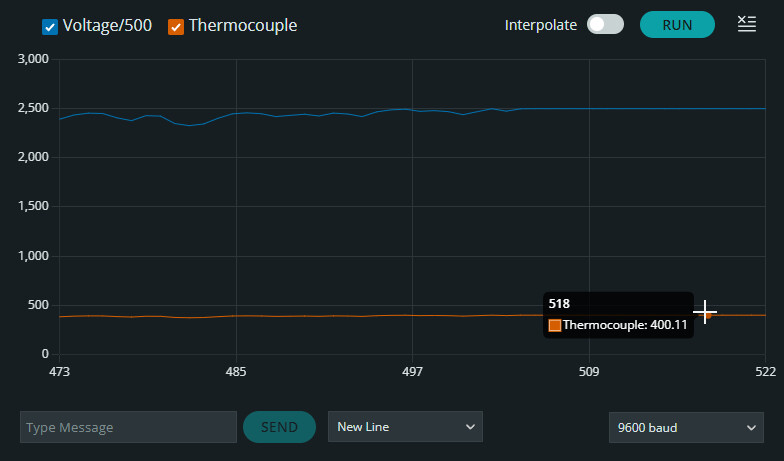
\includegraphics[width=\linewidth]{thermocouple_temp.jpg}
    \caption{Графік нагрітої термопари}
    \label{fig:plot_station}
\end{figure}
